%(BEGIN_QUESTION)
% Copyright 2007, Tony R. Kuphaldt, released under the Creative Commons Attribution License (v 1.0)
% This means you may do almost anything with this work of mine, so long as you give me proper credit

Anta at kraftspolen i denne strøm-til-trykk (I/P)-omformeren plutselig får avbrudd (åpen krets):

$$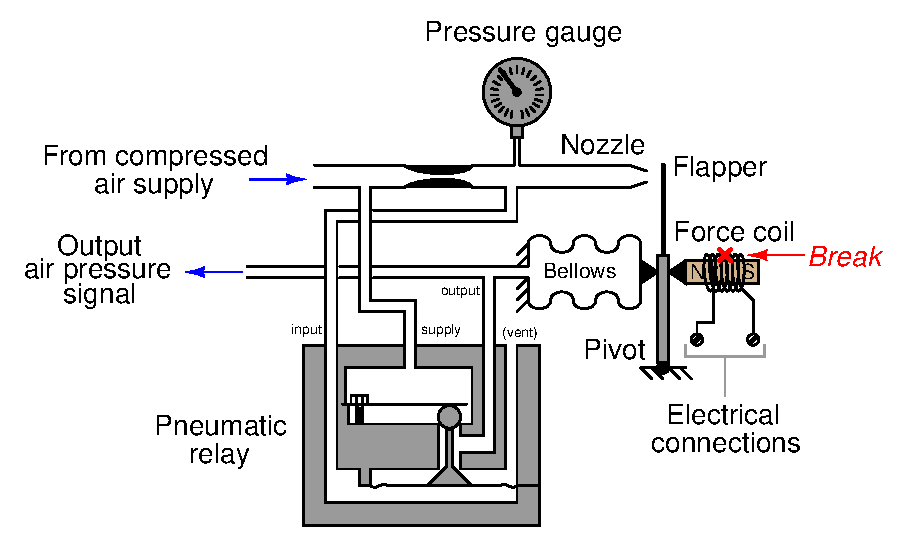
\includegraphics[width=15.5cm]{i01618x01.eps}$$

\noindent
Velg det beste svaret som beskriver virkningene av denne feilen:

\begin{itemize}
\item{} Utgangstrykket vil falle helt ned til 0 PSI
\vskip 10pt
\item{} Utgangstrykket vil øke litt
\vskip 10pt
\item{} Utgangstrykket vil stige helt opp til fullt forsyningstrykk (PSI)
\vskip 10pt
\item{} Utgangstrykket vil avta litt
\vskip 10pt
\item{} Det vil ikke ha noen effekt overhodet -- alt fortsetter som normalt
\end{itemize}


\underbar{file i01618}
%(END_QUESTION)





%(BEGIN_ANSWER)

Utgangstrykket vil falle helt ned til 0 PSI

%(END_ANSWER)





%(BEGIN_NOTES)

{\bf Dette spørsmålet er kun ment for eksamen, ikke arbeidsark!}.

%(END_NOTES)
